\appendix

\chapter{流体与定温热源的传热计算公式}
假定$U$,$T_{c}$,$\dot{m}$和$c_{p}$都为常数,对于给定的来流温度$T_{i}$,
\nomenclature[S]{$i$}{入口}

\noindent \begin{center}
\begin{figure}[h]
\begin{centering}
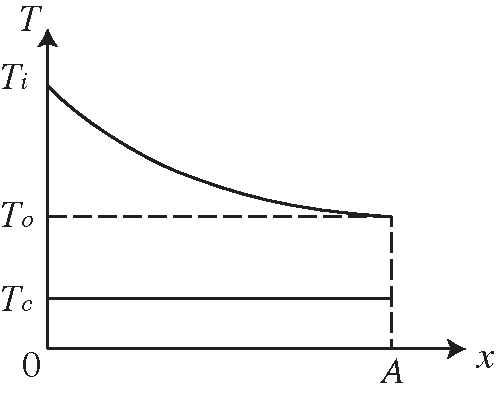
\includegraphics[width=0.4\textwidth]{fig/ConstTempHX.pdf}
\par\end{centering}
\caption{流体与定温热源的传热示意图}
\label{fig:CTHX}
\end{figure}
\par\end{center}

取$x$为已经参与换热的面积,当$x=0$时,$T(x)=T_i$;当$x=A$时,$T(x)=T_o$。
\nomenclature[S]{$o$}{出口}

\begin{equation}
\dot{m}c_{p}dT(x)=(T_{c}-T(x))Udx
\end{equation}

于是,

\begin{equation}
\frac{dT(x)}{dx}=-\frac{U}{\dot{m}c_{p}}(T(x)-T_{c})
\end{equation}

\begin{equation}
T_{g}(x)=T_{p}(x)+T_{h}(x)
\end{equation}

其中,$T_{g}(x)$是通解,$T_{p}(x)$是特解,$T_{h}(x)$是齐次解。

\begin{equation}
-\frac{U}{\dot{m}c_{p}}(T_{p}(x)-T_{c})=0
\end{equation}

\begin{equation}
T_{p}(x)=T_{c}
\end{equation}

\begin{equation}
\frac{dT_{h}(x)}{dx}=-\frac{U}{\dot{m}c_{p}}T_{h}(x)\label{eq:T_h(x)}
\end{equation}

\begin{equation}
\int_{T_{h}(x)=T_{h}(0)}^{T_{h}(x)=T_{h}(A)}\frac{dT_{h}(x)}{T_{h}(x)}=-\int_{x=0}^{x=A}\frac{U}{\dot{m}c_{p}}dx
\end{equation}
\begin{equation}
\frac{T_{h}(A)}{T_{h}(0)}=\exp(-\frac{UA}{\dot{m}c_{p}})
\end{equation}

也就是

\begin{equation}
\frac{T_{g}(A)-T_{p}(A)}{T_{g}(0)-T_{p}(0)}=\exp(-\frac{UA}{\dot{m}c_{p}})
\end{equation}

\begin{equation}
\frac{T_{o}-T_{c}}{T_{i}-T_{c}}=\exp(-\frac{UA}{\dot{m}c_{p}})
\label{eq:Eq}
\end{equation}

\chapter{等热流密度下的流体与定温热源的传热计算公式}
\label{cha:CTCHFHX}

假定$U$,$T_{c}$,$\dot{m}$,$c_p$和$q''$都为常数,对于给定的来流温度${T_i}$,

\noindent \begin{center}
\begin{figure}[h]
\noindent \begin{centering}
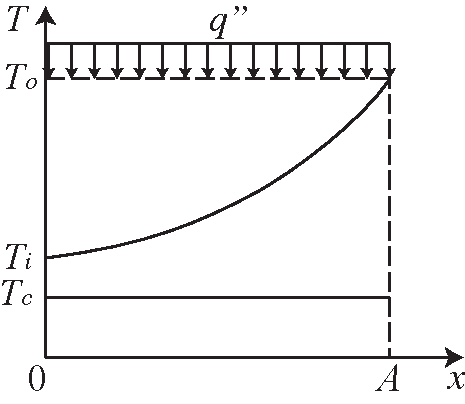
\includegraphics[width=0.4\textwidth]{fig/CTCHFHX.pdf}\caption{等热流密度下的流体与定温热源的传热示意图}
\label{fig:CTCHFHX}
\par\end{centering}
\end{figure}
\par\end{center}

取$x$为已经参与换热的面积,当$x=0$时,$T(x)=T_i$;当$x=A$时,$T(x)=T_o$。
\begin{equation}
\dot{m}c_{p}dT(x)=(T_{c}-T(x))Udx+q''dx
\end{equation}

于是,

\begin{equation}
\frac{dT(x)}{dx}=-\frac{UP}{\dot{m}c_{p}}T(x)+\frac{q''P+UPT_{c}}{\dot{m}c_{p}}
\end{equation}
%\nomenclature[S]{$g$}{通解}
%\nomenclature[S]{$p$}{Particular solution}
%\nomenclature[S]{$h$}{Homogeneous solution}
\begin{equation}
T_{g}(x)=T_{p}(x)+T_{h}(x)
\end{equation}

其中,$T_{g}(x)$是通解,$T_{p}(x)$是特解,$T_{h}(x)$是齐次解。

\begin{equation}
-\frac{U}{\dot{m}c_{p}}T_{p}(x)+\frac{q''+UT_{c}}{\dot{m}c_{p}}=0
\end{equation}

\begin{equation}
T_{p}(x)=T_{c}+\frac{q''}{U}
\end{equation}

\begin{equation}
\frac{dT_{h}(x)}{dx}=-\frac{U}{\dot{m}c_{p}}T_{h}(x)
\end{equation}

同方程(\ref{eq:T_h(x)})一样,于是有
\begin{equation}
\frac{T_{g}(A)-T_{p}(A)}{T_{g}(0)-T_{p}(0)}=\exp(-\frac{UA}{\dot{m}c_{p}})
\end{equation}

\begin{equation}
\frac{T_{o}-T_{c}-\dfrac{q''}{U}}{T_{i}-T_{c}-\dfrac{q''}{U}}=\exp(-\frac{UA}{\dot{m}c_{p}})
\end{equation}

\chapter{类Stream的MATLAB源代码}
\label{cha:MATLAB_SOURCECODE}

%\begin{lstlisting}[language= MATLAB, backgroundcolor = \color{yellow!20}, title = {The MATLAB source code of the definition of the class -- Stream}, label = {lst:MATLAB_SOURCECODE}]
\begin{lstlisting}[language= MATLAB, backgroundcolor = \color{yellow!20}, label = {lst:MATLAB_SOURCECODE}]
classdef Stream < handle
    %Stream This class describes a fluid stream that has inherent
    %properties and dependent properties
    
    properties
        fluid;  % Fluid type
        dot_m;  % Mass flow rate, kg/s
        T;      % Temperature, K
        p;      % Pressure, Pa
        x;      % Quality, [0, 1] for two phase stream; NaN for single 
                %   phase stream
    end
    properties(Dependent)
        h;      % Mass specific enthalpy, J.kg
        s;      % Mass specific entropy, J/kg-K
        cp;     % Specific heat under constant pressure, J/kg-K
    end
    
    methods
        function obj = Stream
            obj.T = Temperature;
            obj.dot_m = Massflow;
            obj.p = Pressure;
        end
        function flowTo(obj, st)
            st.fluid = obj.fluid;
            st.dot_m = obj.dot_m;
        end
        function st2 = mix(obj, st1)
            % Get the properties of a stream mixed by two streams
            % The two streams must have the same fluid type and pressure
            if obj.fluid == st1.fluid
                if  obj.p.v == st1.p.v
                    obj.p = st1.p;
                    st2.fluid = obj.fluid;
                    st2.p = obj.p;
                    st2.dot_m.v = obj.dot_m.v + st1.dot_m.v;
                    h = (obj.dot_m.v .* obj.h + st1.dot_m.v .* st1.h)...
                        ./ (obj.dot_m.v + st1.dot_m.v);
                    st2.T.v = CoolProp.PropsSI('T', 'H', h, 'P',st2.p.v);
                else
                    error('The two streams have different pressures!');
                end
            else
                error('The two streams have different fluid types!');
            end
        end
        function convergeTo(obj, st, y)
            % Get another stream converged (or diverged)
            % from the original stream state.
            % If y < 1, the original stream is diverged
            % If y > 1, the original stream is converged
            st.fluid = obj.fluid;
            st.T = obj.T;
            st.p = obj.p;
            st.x = obj.x;
            st.dot_m.v = obj.dot_m.v .* y;
        end
    end
    methods
        % The dependent properties can be obtained from the inherent
        %   properties
        % If x is NaN, then the dependent properties are determined
        %   by T and P; otherwise, they are determined by P and x
        function value = get.h(obj)
            if isempty(obj.x)
                value = CoolProp.PropsSI('H', 'T', obj.T.v, ...
                    'P', obj.p.v, obj.fluid);
            else
                value = CoolProp.PropsSI('H', 'P', obj.p.v, 'Q', ...
                    obj.x, obj.fluid);
            end
        end
        function value = get.s(obj)
            if isempty(obj.x)
                value = CoolProp.PropsSI('S', 'T', obj.T.v, ...
                    'P', obj.p.v, obj.fluid);
            else
                value = CoolProp.PropsSI('S', 'P', obj.p.v, 'Q', ...
                    obj.x, obj.fluid);
            end
        end
        function value = get.cp(obj)
            if isempty(obj.x)
                value = CoolProp.PropsSI('C', 'T', obj.T.v, ...
                    'P', obj.p.v, obj.fluid);
            else
                value = inf;
            end
        end
    end
end
\end{lstlisting}
%\chapter{Stirling engine model}\label{sec:Stirling-engine-model}
%
%A simple Stirling engine model is used for the system. The cycle efficiency is given by \cite{Stine1985}
%
%\begin{equation}
%	\eta=\frac{T_{H}-T_{L}}{T_{H}+\text{\ensuremath{\dfrac{1-e}{k-1}}}\cdot\dfrac{T_{H}-T_{L}}{\ln\gamma}}\label{eq:eta_stirling}
%\end{equation}
%
%
%where \nomenclature{$e$}{Regeneration effectiveness of the Stirling engine}$e = (T_{R}-T_{L}) / (T_{H}-T_{L})$,\nomenclature{$T_R$}{Regenerator temperature, K}$T_{R}$ is the\emph{ }regenerator temperature, \nomenclature{$c_p$}{Heat capacity of Stirling engine working gas at constant pressure, J/(kg$\cdot$K)}\nomenclature{$c_v$}{Heat capacity of Stirling engine working gas at constant volume, J/(kg$\cdot$K)}$k=c_{p}/c_{v}$ for the working gas, $\gamma_{se}=V_{max}/V_{min}$ is the compression ratio.
%
%The heat transfer diagram is shown in Figure~\ref{fig:Heat-transfer-diagram}. Flow 1 is used for heating the hot chamber of Stirling engine, $T_{1i}$ is the inlet temperature, $T_{1o}$ is the outlet temperature. Flow 2 is used for cooling the cold chamber of Stirling engine, $T_{2i}$ is the inlet temperature, $T_{2o}$ is the outlet temperature. \nomenclature{$T_H$}{Highest temperature of expansion space, K}$T_{H}$ is the highest temperature of expansion space, \nomenclature{$T_L$}{Lowest temperature of compression space, K}$T_{L}$ is the lowest temperature of compression space.
%
%\noindent \begin{center}
%\begin{figure}[h]
%	\noindent \centering{}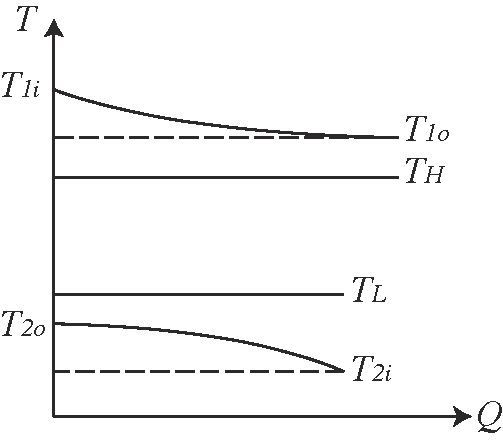
\includegraphics[width=0.4\columnwidth]{fig/StirilingHT}
%	\protect\caption{\label{fig:Heat-transfer-diagram}Heat transfer diagram of Stirling
%engine}
%\end{figure}
%
%\par\end{center}
%
%According to Equation (\ref{eq:Eq}),
%
%\begin{equation}
%	\dfrac{T_{1o}-T_{H}}{T_{1i}-T_{H}}=\exp(-\dfrac{U_{1}A_{1}}{\dot{m}_{1}c{}_{p1}})
%\end{equation}
%
%and
%
%\begin{equation}
%	\dfrac{T_{2o}-T_{L}}{T_{2i}-T_{L}}=\exp(-\dfrac{U_{2}A_{2}}{\dot{m}_{2}c_{p2}})
%\end{equation}
%
%So known $T_{1o},T_{1i},U_{1},A_{1},\dot{m}_{1},c_{p1},T_{2o},T_{2i},U_{2},A_{2},\dot{m}_{2},c_{p2}$, $T_{H}$ and $T_{L}$ can be calculated, and then $\eta$ can be obtained by using Equation (\ref{eq:eta_stirling}).
%\nomenclature{$A$}{Area, m$^2$}
  
\begin{publications}
  \item Cheng Zhang, Yanping Zhang, Inmaculada Arauzo, Wei Gao, Chongzhe  Zou. Cascade system using both trough system and dish system for power generation. Energy Conversion and Management. 2017.06.15;142:494–503.
  \item Cheng Zhang, Yanping Zhang, Xiaolin Lei, Wei Gao. Design and Comparison of Solar Thermal Oilfield Steam Production System Plans. Journal of Solar Energy Engineering. 2017.01.08;139;004502-4.
  \item Cheng Zhang, Kun Wang, Jizhou Wang, Shuhong Huang. FEA simulation on the alignment of the shafts of three-fulcrum turbine. International Conference on Power Engineering. 2013.
  \item Chongzhe Zou, Yanping Zhang, Quentin Falcoz, Pierre Neveu, Cheng Zhang, Shuhong Huang, Weicheng Shu. Design and Optimization of a High-temperature Cavity Receiver for a Solar Energy Cascade Utilization System. Renewable Energy. 2017.04.01:103; 478-89. 
  \item Chongzhe Zou, Yanping Zhang, Huayi Feng, Quentin Falcoz, Pierre Neveu, Cheng Zhang, Wei Gao. “Effects of Geometrical Parameters on Thermal Performance for a Cylindrical Solar Receiver Using 3D numerical Model.” Energy Conversion and Management, 2017.10.1: 126-17.
  \item Chongzhe Zou, Yanping Zhang, Quentin Falcoz, Pierre Neveu,Cheng Zhang. Thermal modeling of a pressurized air cavity receiver for solar dish Stirling system, Solarpaces: International Conference on Concentrating Solar Power \& Chemical Energy Systems. AIP Publishing LLC, 2017:1884-1892.
  
  \item A solar thermal cascade system, No. 201610806296.5
  \item A flow control method used in a multistage heating system, No. 201610805604.2
  
\end{publications}